%!TEX TS-program = xelatex
%!TEX encoding = UTF-8 Unicode

\documentclass[12pt, A4]{article}
\usepackage[utf8]{inputenc}

%%%%%% Font setting %%%%%%

\usepackage{fontspec} %加這個就可以設定字體 

\usepackage{xeCJK} %讓中英文字體分開設置
%\setmainfont{Apple Symbols}
\setCJKmainfont{STKaiti} %設定中文為系統上的字型,而英文不去更動,使用原TeX字型
%\setmonofont{Courier} %等寬字體
\setmonofont{Oxygen Mono}

\XeTeXlinebreaklocale "zh" %這兩行一定要加,中文才能自動換行
\XeTeXlinebreakskip = 0pt plus 1pt 

%%%%%% Coding style %%%%%%
% sudo easy_install Pygments
% Add -shell-escape to compile flag
\usepackage{minted}

% Run in terminal for checking available styles: pygmentize -L styles
\usemintedstyle{friendly}

\usepackage{hyperref}


%%%%%% 文件正式開始 %%%%%%

\title{Compiler \\ Assignment 3 \\ Automatic Conversion from Regular Expressions to Finite Automata}
\author{403410033 \ 資工三 \ 曾俊宏}
\date{\today}

\begin{document}
	
	\maketitle

	\section{Question 1}
	
	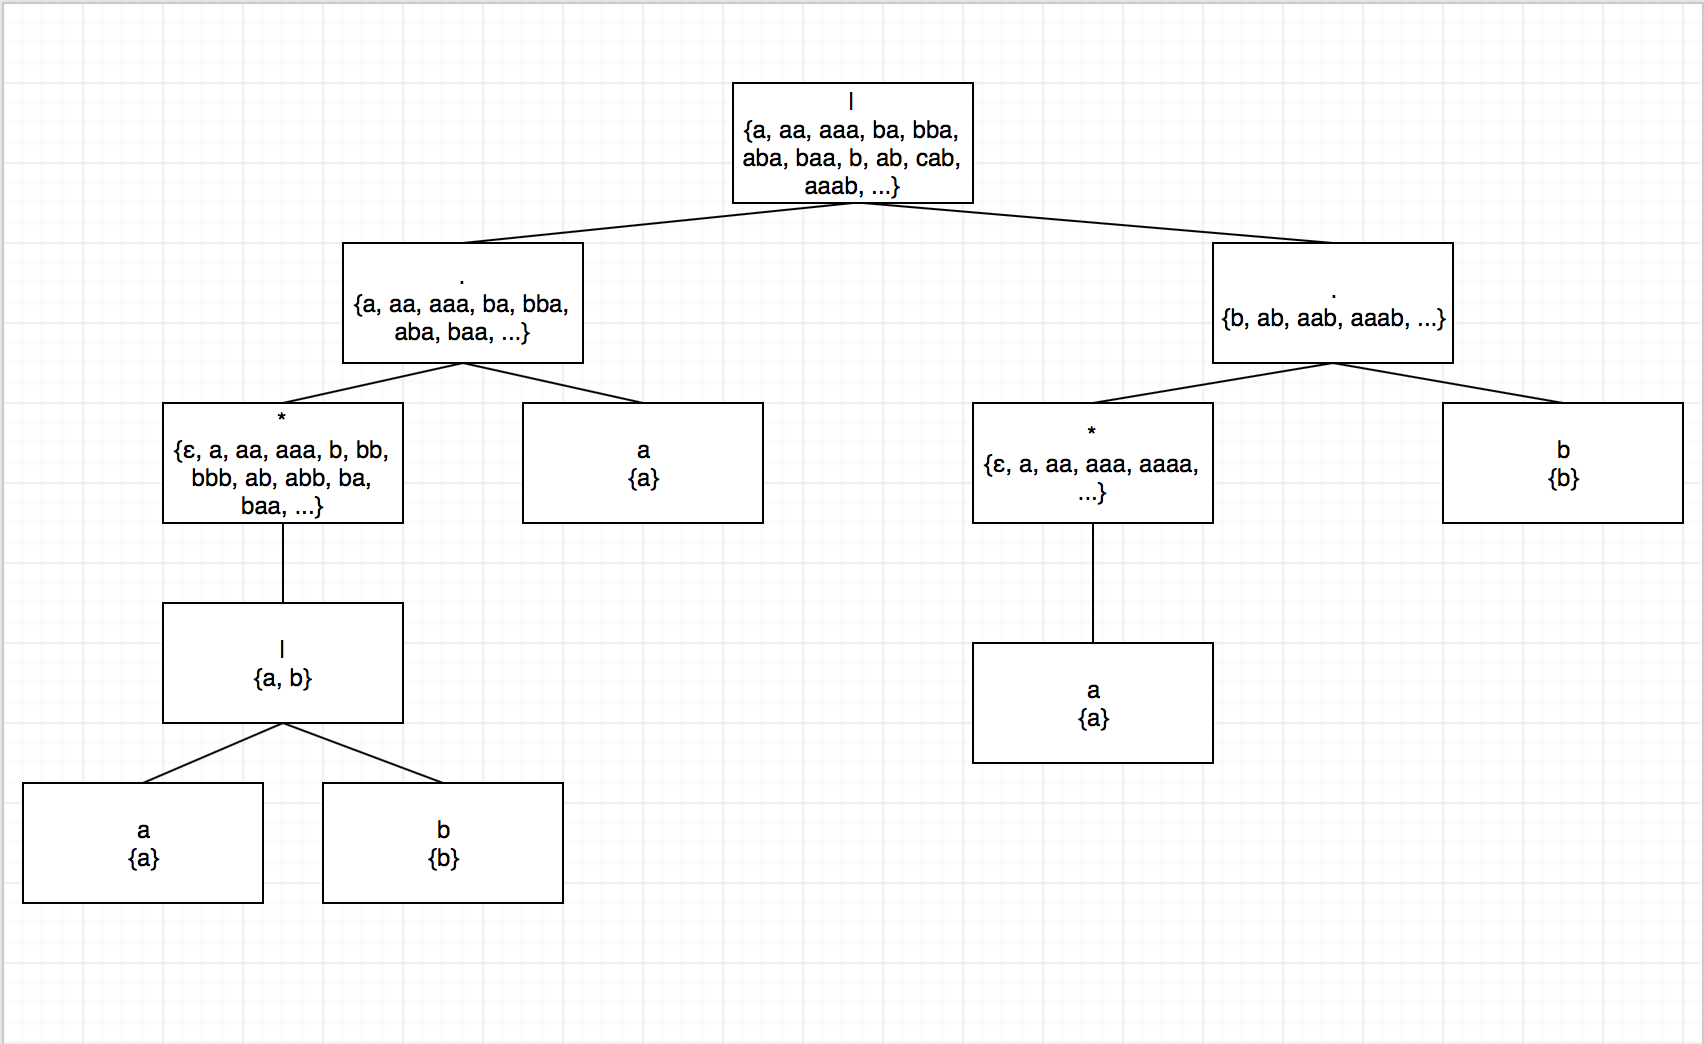
\includegraphics[scale=0.55]{Question1}
	
	\newpage
	
	\section{Question 2}
	
	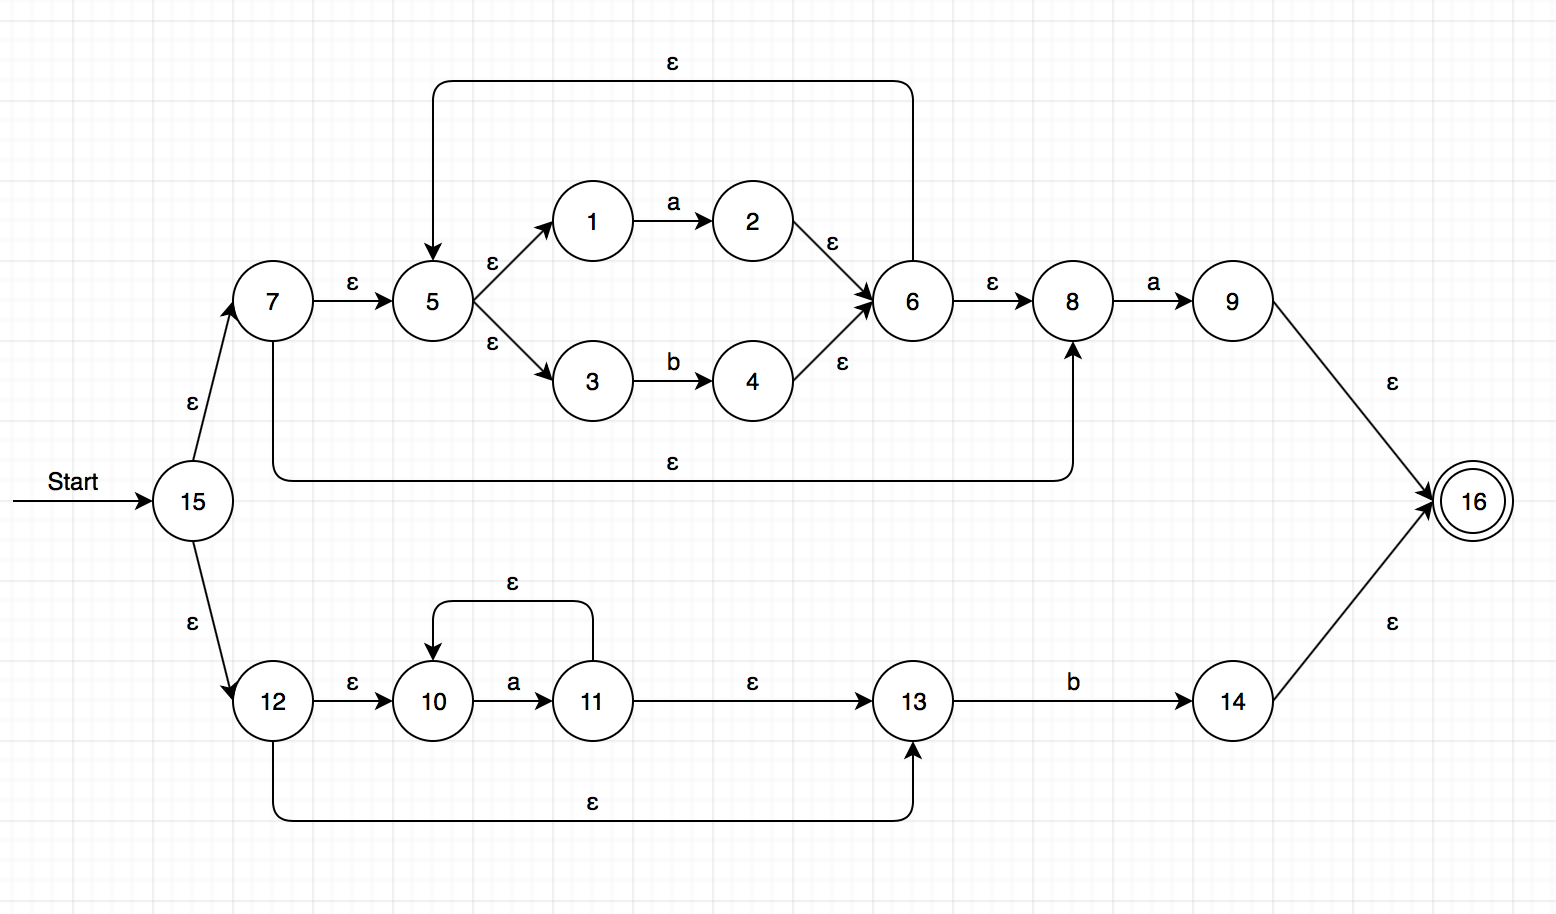
\includegraphics[scale=0.6]{Question2}
	
	\newpage
	
	\section{Question3}
	
	$S_0$ = $\epsilon-closure(\{15\}) \\= \{1, 3, 5, 7, 8, 10, 12, 13, 15\} = A$\\ \\
	$S_1$ = $\epsilon-closure(move(A, a)) \\= \epsilon-closure(\{2, 9, 11\}) \\= \{1, 2, 3, 5, 6, 8, 9, 10, 11, 13, 16\} = B$\\ \\
	$S_2$ = $\epsilon-closure(move(A, b)) \\= \epsilon-closure(\{4, 14\}) \\= \{1, 3, 4, 5, 6, 8, 14, 16\} = C$\\ \\
	$S_3$ = $\epsilon-closure(move(B, a)) \\= \epsilon-closure(\{2, 9, 11\}) = D$\\ \\
	$S_4$ = $\epsilon-closure(move(B, b)) \\= \epsilon-closure(\{4, 14\}) = C$\\ \\
	$S_5$ = $\epsilon-closure(move(C, a)) \\= \epsilon-closure(\{2, 9\}) \\= \{1, 2, 3, 5, 6, 8, 9, 16\} = D$\\ \\
	$S_6$ = $\epsilon-closure(move(C, b)) \\= \epsilon-closure(\{4\}) \\= \{1, 3, 4, 5, 6, 8\} = E$\\ \\
	$S_7$ = $\epsilon-closure(move(D, a)) \\= \epsilon-closure(\{2, 9\}) = D$\\ \\
	$S_8$ = $\epsilon-closure(move(D, b)) \\= \epsilon-closure(\{4\}) = E$\\ \\
	$S_9$ = $\epsilon-closure(move(E, a)) \\= \epsilon-closure(\{2, 9\}) = D$\\ \\
	$S_{10}$ = $\epsilon-closure(move(E, b)) \\= \epsilon-closure(\{4\}) = E$\\
	
	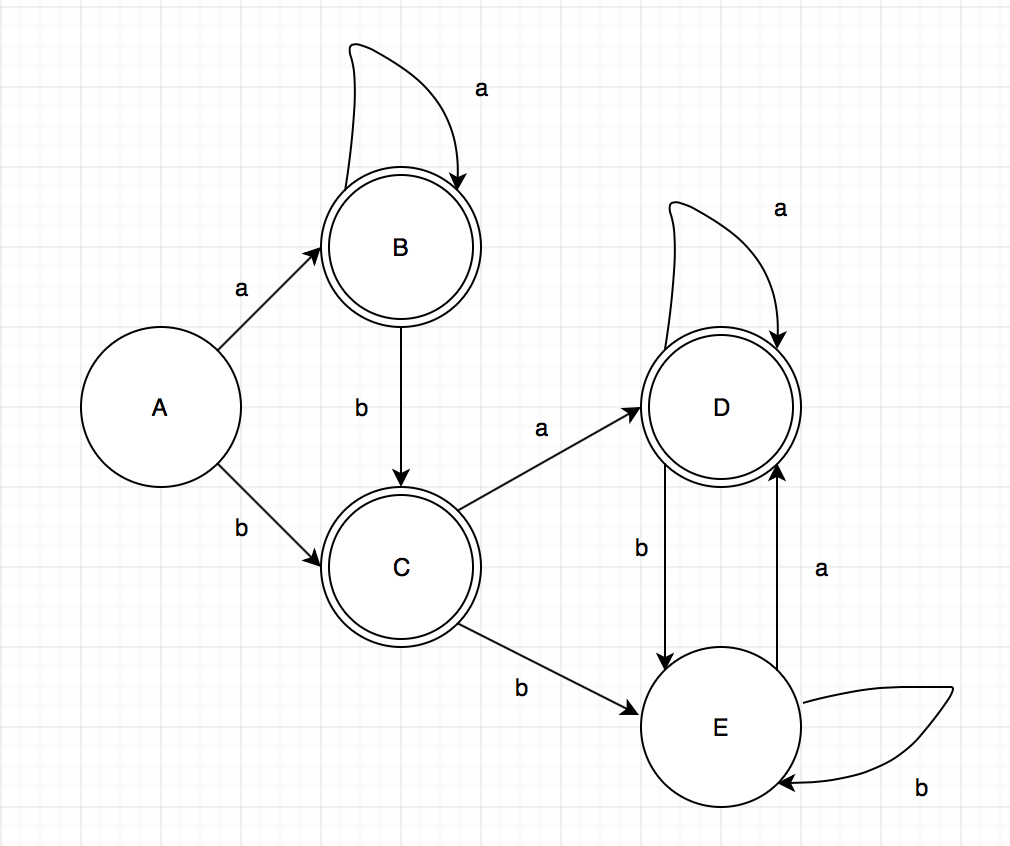
\includegraphics[scale=0.8]{Question3}
	
\end{document}